\documentclass{article}
\usepackage{tikz}
\usetikzlibrary{arrows.meta,positioning,calc,shapes.geometric}
\pagestyle{empty}
\begin{document}
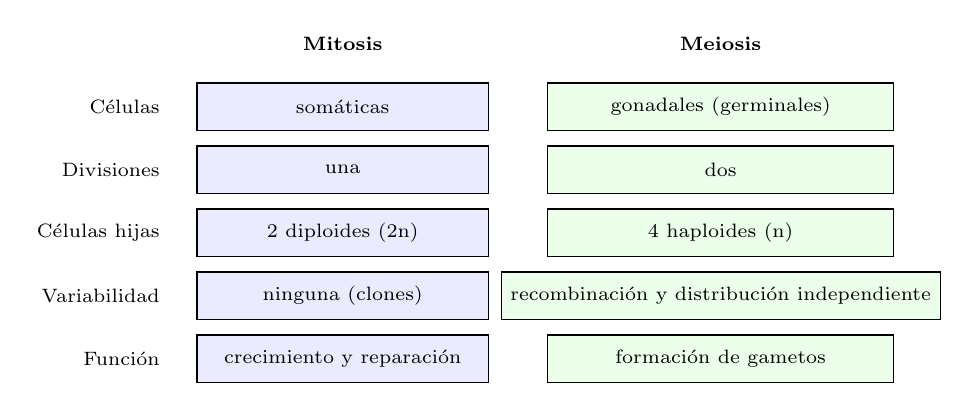
\begin{tikzpicture}

\node[font=\bfseries\scriptsize] at (3.6,4.3) {Mitosis}; \node[font=\bfseries\scriptsize] at (8.4,4.3) {Meiosis};
\foreach \y/\l/\a/\b in {3.5/Células/somáticas/gonadales (germinales), 2.7/Divisiones/una/dos, 1.9/Células hijas/2 diploides (2n)/4 haploides (n), 1.1/Variabilidad/ninguna (clones)/recombinación y distribución independiente, 0.3/Función/crecimiento y reparación/formación de gametos} {
  \node[font=\scriptsize, left] at (1.4,\y) {\l}; \node[draw, fill=blue!8, minimum width=3.7cm, minimum height=0.6cm, font=\scriptsize] at (3.6,\y) {\a}; \node[draw, fill=green!8, minimum width=4.4cm, minimum height=0.6cm, font=\scriptsize] at (8.4,\y) {\b};}

\end{tikzpicture}
\end{document}
